\documentclass{article}
\usepackage[preprint]{neurips_2023}
\usepackage[utf8]{inputenc} % allow utf-8 input
\usepackage[T1]{fontenc}    % use 8-bit T1 fonts
\usepackage{hyperref}       % hyperlinks
\usepackage{url}            % simple URL typesetting
\usepackage{booktabs}       % professional-quality tables
\usepackage{amsfonts}       % blackboard math symbols
\usepackage{nicefrac}       % compact symbols for 1/2, etc.
\usepackage{microtype}      % microtypography
\usepackage{xcolor}         % colors
\usepackage{graphicx}
\usepackage{float} 
\usepackage{subfigure}
\title{Final report for AI project - Tank War}

\author{
  liupch1 \\
  \texttt{liupch1@shanghaitech.edu.cn}\\
      \AND
  chjl \\
  \texttt{chenjl1@shanghaitech.edu.cn}\\ 
      \AND 
  gujq  \\
  \texttt{gujq@shanghaitech.edu.cn}  
}

\begin{document}
	
	\maketitle
	
	\begin{abstract}
		The purpose of the project is to solve the core issues of Tank War (with simplified game environment and rules ) - protecting the base camp, avoiding obstacles, and defeating opponents. This code mainly tests the offline search algorithm, targeting opponents of three different difficulty levels, and achieving results in different situations that emphasize aggression and defense.
	\end{abstract}
	
	
	\section{Simplification of game environment}
	\begin{figure}[H]
		\centering
		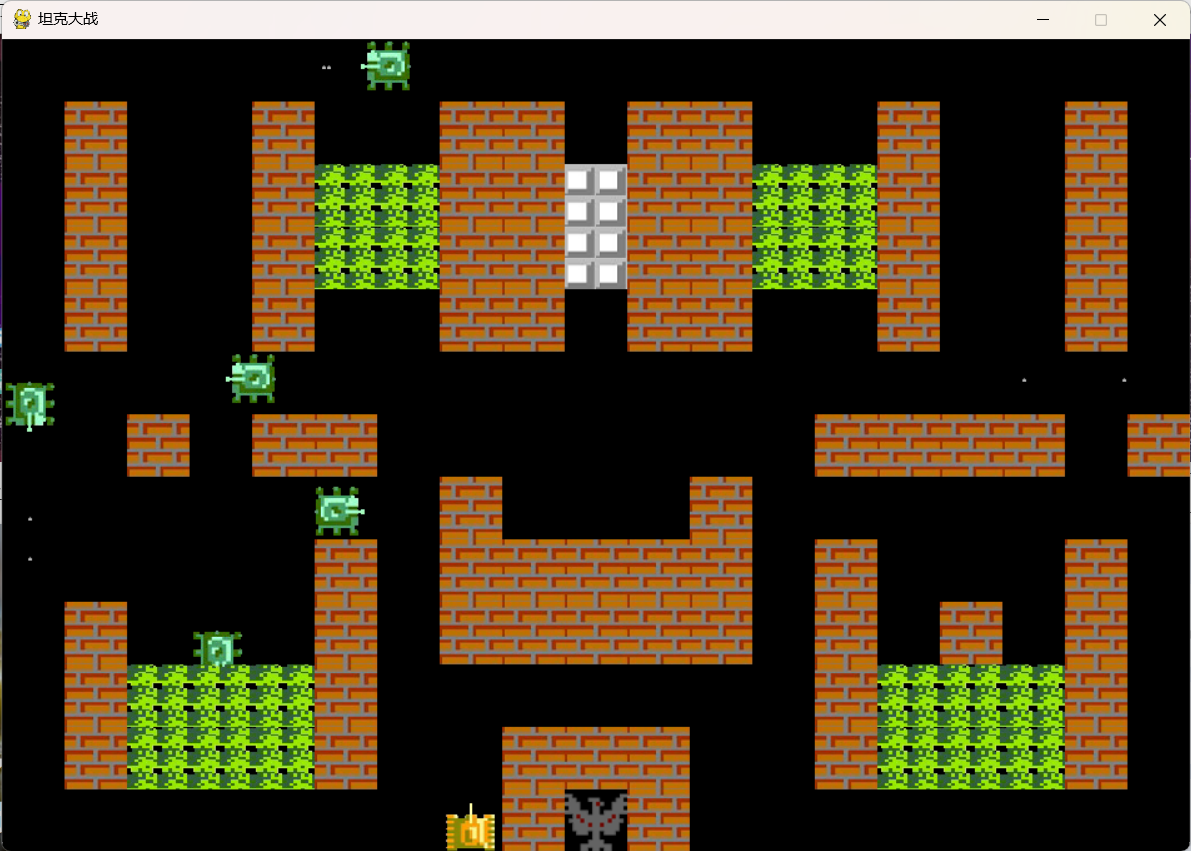
\includegraphics[width=0.7\textwidth]{game.png}
		\caption{Tank war}
	\end{figure} 
	Environment:\\
	1.Variable wall with different blood -- fixed maze per game with unbreakable walls \\
	2.The maze is randomly generated in the case of walls with a 20\% grid ratio, excluding cases that any tank being besieged or unable to search for a path to the base camp.\\
	\space\\
	Agent:\\
	1.picture of tanks with a certain area -- circles occupying the size of one grid \\
	2.Hero tank (red) and enemy tank (blue) share the same speed (one grid per time)\\
	3.Use bullets to defeat opponents -- Defeat opponents through collisions\\
	
	Time limit:\\
	1.Controlled by points, excluding attacks or defeats on the base camp, the game ends with a deduction of points per step when testing the offensive strategy. Points less than or equal to -100 are added per step when testing the defensive strategy, and points greater than 250 are added per step when the game ends.\\
	
	\begin{figure}[H]
		\centering
		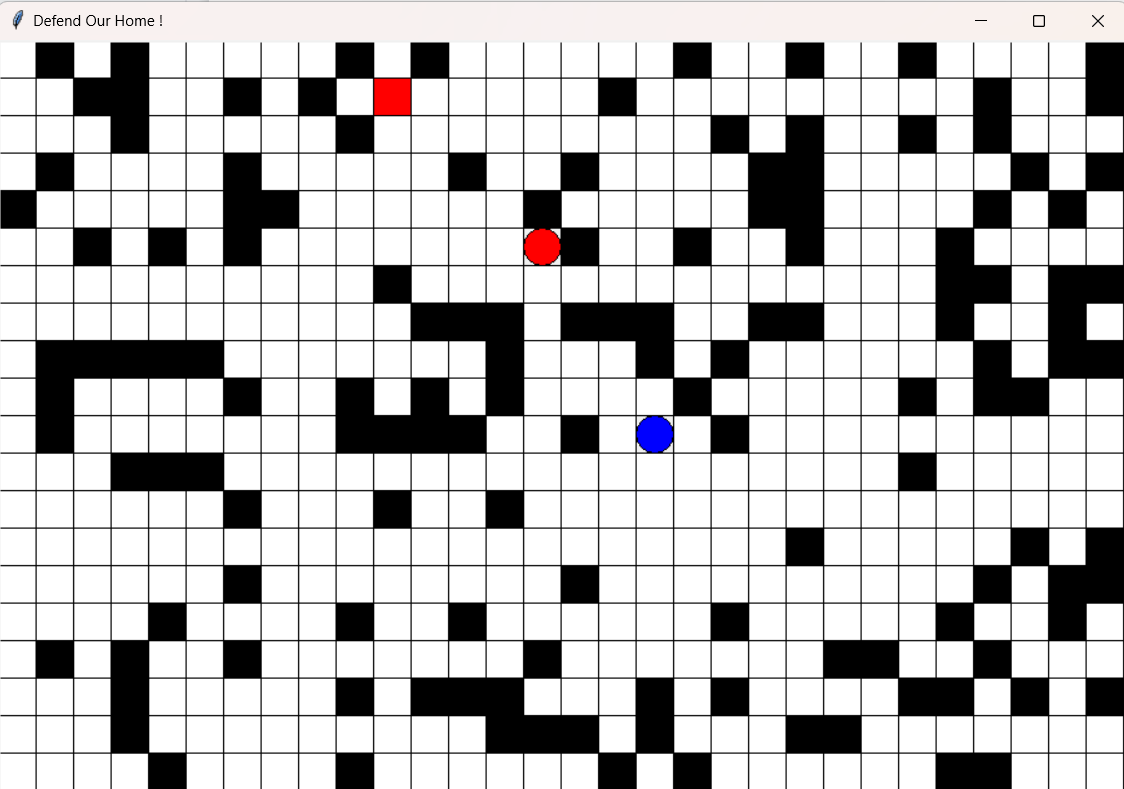
\includegraphics[width=0.7\textwidth]{simplified.png}
		\caption{Simplified game}
	\end{figure} 

	Due to these simplifications, there is no midway reward in game. We judge that the offline strategy is suitable for this task.\\
		

\section{Strategy}
\label{gen_inst}
All the distance mentioned means manhattan distance:\\
abs(current position.row - end position.row) + abs(curr position.col - end position.col)\\
\subsection{Enemy Agent(Blue Agent, also called Target)}
Agent1.move randomly with preference:\\
Random movement without hitting the wall. \\
Since we know where the Red Square is , we can set a prefenrence of moving up and left.\\
In the final submitted code, the value used to set preferences is set to 0.5, which is completely random\\

Agent2.move along a fixed path :\\
 Using the breadth-first algorithm(bfs) or A-star algorithm(A*) to find the shortest path to the Red Square headquarters.\\
 
Agent3.avoid clutches and make an attack:\\
1.When the distance between Red and Blue is greater than the threshold(safe) or Blue is closer to the Red Square than Red(Blue win when moving optimally) ,approaching the Red Square throurg the optimal path found by A *, and vice versa, the priority is to stay away from Red.\\
The threshold is 6 then 2 during the game, meaning Blue take braber action when the game is over halfway.\\
2.When Blue is closer to the Red Square than Red(Blue win when moving optimally) , approaching the Red Square throurg the optimal path found by A *\\
A* complexity:O(mn)*log(mn)\\



\subsection{Hero Agent(Red Agent, also called Agent)}
Agent1:using BFS to chase enemy\\
Complexity: O(mn)\\

Agent2:Knowing the enemy's strategy and iterating through each cell on the enemy's optimal path to obtain the cells that one can reach simultaneously with it, and using BFS to reach this cell. (optimal)\\

Agent3:Patrol within a distance of 8 units around home. Taking Agent2 when meeting the requirements.It's because our intuition that moving around home during defense is less likely to be attacked and may result in higher scores.\\

\section{Result}
\label{others}
We proved that agent2 is already optimal for enemies taking different strategies listed above through the following process.\\

Win:Collision occured\\
Loss:Attack occurred\\
draw:No collision or attack occurred\\

Scoring Criteria 1 - aggression:\\
score =\\
100*(Red and Blue collide)\\
-100*(home attacked)\\
-1 * step \\

1. red(agent1) vs blue(random)
500 games, 6 draws, with an average score of 52.17.\\
Draws were caused by random movements of enemy.\\

2.red(agent2) vs. blue(fixed path)
500 games, 7 lossed, with an average score of 72.84.\\
Losses were caused by random generated maze.(Blue is closer to the Red Square than Red at the beginning.)\\

3.red(agent1 to agent2) vs. blue(Agent3):\\
The first n steps take agent2, and the next n steps take agent1.The following figure shows that when agent2 is used throughout the game, the score is highest. However, the highest is still a negative value.\\
	\begin{figure}[H]
	\centering
	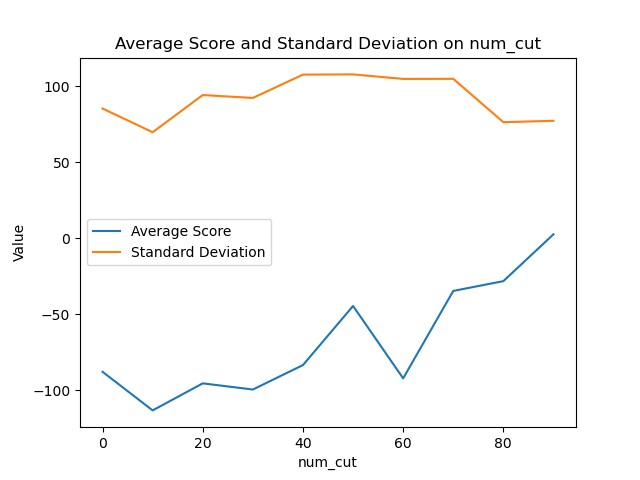
\includegraphics[width=0.7\textwidth]{r1.png}
	\caption{red(agent1 to agent2) vs. blue(Agent3)}
	\end{figure} 

After observing the game process through the visual interface, we found that this was due to many draws and the penalty points for each step during the draw.\\
But from the perspective of defending our home , persisting longer should receive rewards.\\
Hence we design the second score Criteria.\\


Scoring Criteria 2 - defense:\\
score =\\
300*(Red and Blue collide)\\
-300*(home attacked)\\
+0.5 * step(Red and Blue collidision is equivalent to protecting the home throughout the whole game, this part will take the maximum step value) \\

1.red(agent1 to agent2) vs. blue(Agent3):\\
The first n steps take agent2, and the next n steps take agent1. We see smaller standard deviations than the score, showing that the results are more interpretable.\\
	\begin{figure}[H]
	\centering
	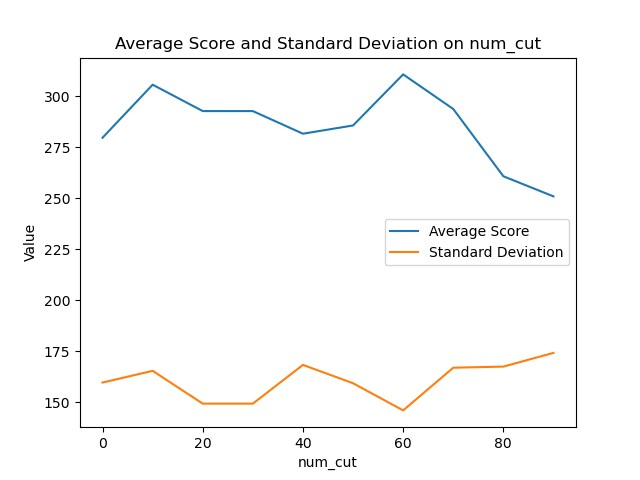
\includegraphics[width=0.7\textwidth]{r2.png}
	\caption{red(agent1 to agent2) vs. blue(Agent3)}
\end{figure} 
When emphasizing defense, there is no significant and regular difference in the scores brought by Agent1 and Agent2.\\

2.red(agent2) vs. blue(Agent3):\\
500 games with an average score of 287.165\\

3.red(agent3) vs. blue(Agent3):\\
500 games with an average score of 69.5\\

Average score more than 250 means that most time hero tank defeat the enemy tank and get the 300 reward. 69.5 shows that usually hero can protect home but can't defeat the enemy.

Above all, we have proved that agent2 is optimal among strategies we listed when meeting different enemies.

Other-Enemy Agent3:\\
For Blue , taking high-risk measures too early is clearly disadvantageous. We can see under the scoring criteria 1 , right after Blue change from agent3 to agent2(taking risking action), it was caught by Red.\\

	\begin{figure}[H]
	\centering
	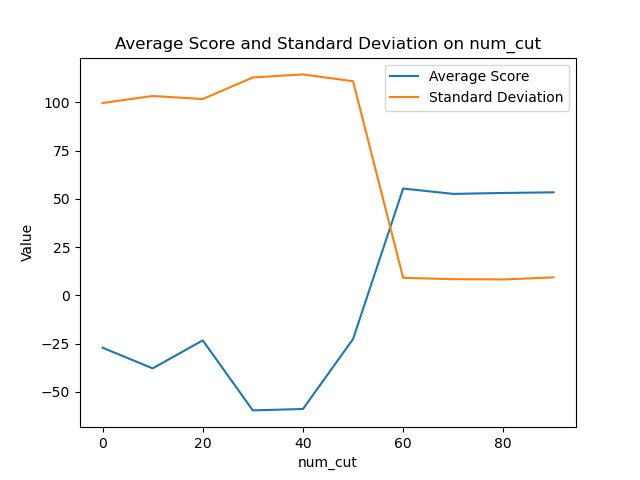
\includegraphics[width=0.7\textwidth]{r3.png}
	\caption{red(agent1 to agent2) vs. blue(Agent3)}
\end{figure} 

For further exploration, if we consider more on Blue's side, we can find better ways to balance parameters for evasion and attack.
If we consider more on Red's side, we should consider situations when we don't know the enemy's strategy , has 2 enemies, or has food and props in the maze.\\


\section{Division Of Labour}
Primary contributor: \\
Pengcheng Liu:\\
Overall framework construction\\
Hero Agent Algorithm\\
Aggression scoring criteria\\
Multi threaded result collector\\
Debug\\
Readme.md\\

Second contributor: \\
Jianglian Chen:\\
Enemy agent\\
Defense scoring criteria\\
Debug\\
Presentation\\
Final report\\

Third contributor: \\
Jiaqi Gu\\
None after simplification (did not commit even once).  
Furthermore did not check others' commit until the day before final presentation.
It wasn't until the afternoon before the final presentation that he started asking how to use the MainGame.py \\
However, he \textbf{truely} did commit once for the old framework, which just includes some naive implementations like greedy but didn't consider 
walls clearly and would never work properly. But at his strong request, we post the commit history of the github repository here:

\href{https://github.com/23776301/CS181PJ/commits/main}{https://github.com/23776301/CS181PJ/commits/main}
\begin{ack}
	Our initial framework was found at \href{https://github.com/IronSpiderMan/TankWar}{https://github.com/IronSpiderMan/TankWar}, but after some exploration 
	we found strange bugs in it and then created our own framework from scratch using python GUI tool kinter.
	We just get some inspirations and ideas from this game framework, and
	our final code is actually completely constructed by our own.
\end{ack}
\end{document}